% ARTICLE 2 ----
% This is just here so I know exactly what I'm looking at in Rstudio when messing with stuff.
% Options for packages loaded elsewhere
\PassOptionsToPackage{unicode}{hyperref}
\PassOptionsToPackage{hyphens}{url}
\PassOptionsToPackage{dvipsnames,svgnames*,x11names*}{xcolor}
%
\documentclass[
  11pt,
]{article}
\usepackage{lmodern}
\usepackage{amssymb,amsmath}
\usepackage{ifxetex,ifluatex}
\ifnum 0\ifxetex 1\fi\ifluatex 1\fi=0 % if pdftex
  \usepackage[T1]{fontenc}
  \usepackage[utf8]{inputenc}
  \usepackage{textcomp} % provide euro and other symbols
\else % if luatex or xetex
  \usepackage{unicode-math}
  \defaultfontfeatures{Scale=MatchLowercase}
  \defaultfontfeatures[\rmfamily]{Ligatures=TeX,Scale=1}
\fi
% Use upquote if available, for straight quotes in verbatim environments
\IfFileExists{upquote.sty}{\usepackage{upquote}}{}
\IfFileExists{microtype.sty}{% use microtype if available
  \usepackage[]{microtype}
  \UseMicrotypeSet[protrusion]{basicmath} % disable protrusion for tt fonts
}{}
\makeatletter
\@ifundefined{KOMAClassName}{% if non-KOMA class
  \IfFileExists{parskip.sty}{%
    \usepackage{parskip}
  }{% else
    \setlength{\parindent}{0pt}
    \setlength{\parskip}{6pt plus 2pt minus 1pt}
    }
}{% if KOMA class
  \KOMAoptions{parskip=half}}
\makeatother
\usepackage{xcolor}
\IfFileExists{xurl.sty}{\usepackage{xurl}}{} % add URL line breaks if available
\urlstyle{same} % disable monospaced font for URLs
\usepackage[margin=1in]{geometry}
\usepackage{longtable,booktabs}
% Correct order of tables after \paragraph or \subparagraph
\usepackage{etoolbox}
\makeatletter
\patchcmd\longtable{\par}{\if@noskipsec\mbox{}\fi\par}{}{}
\makeatother
% Allow footnotes in longtable head/foot
\IfFileExists{footnotehyper.sty}{\usepackage{footnotehyper}}{\usepackage{footnote}}
\makesavenoteenv{longtable}
\usepackage{graphicx}
\makeatletter
\def\maxwidth{\ifdim\Gin@nat@width>\linewidth\linewidth\else\Gin@nat@width\fi}
\def\maxheight{\ifdim\Gin@nat@height>\textheight\textheight\else\Gin@nat@height\fi}
\makeatother
% Scale images if necessary, so that they will not overflow the page
% margins by default, and it is still possible to overwrite the defaults
% using explicit options in \includegraphics[width, height, ...]{}
\setkeys{Gin}{width=\maxwidth,height=\maxheight,keepaspectratio}
% Set default figure placement to htbp
\makeatletter
\def\fps@figure{htbp}
\makeatother
\setlength{\emergencystretch}{3em} % prevent overfull lines
\providecommand{\tightlist}{%
  \setlength{\itemsep}{0pt}\setlength{\parskip}{0pt}}
\setcounter{secnumdepth}{5}

\ifluatex
  \usepackage{selnolig}  % disable illegal ligatures
\fi
\newlength{\cslhangindent}
\setlength{\cslhangindent}{1.5em}
\newlength{\csllabelwidth}
\setlength{\csllabelwidth}{3em}
\newenvironment{CSLReferences}[2] % #1 hanging-ident, #2 entry spacing
 {% don't indent paragraphs
  \setlength{\parindent}{0pt}
  % turn on hanging indent if param 1 is 1
  \ifodd #1 \everypar{\setlength{\hangindent}{\cslhangindent}}\ignorespaces\fi
  % set entry spacing
  \ifnum #2 > 0
  \setlength{\parskip}{#2\baselineskip}
  \fi
 }%
 {}
\usepackage{calc}
\newcommand{\CSLBlock}[1]{#1\hfill\break}
\newcommand{\CSLLeftMargin}[1]{\parbox[t]{\csllabelwidth}{#1}}
\newcommand{\CSLRightInline}[1]{\parbox[t]{\linewidth - \csllabelwidth}{#1}\break}
\newcommand{\CSLIndent}[1]{\hspace{\cslhangindent}#1}


\title{Disagreement and dissent on a bench: a quantitative empirical
analysis of the Czech Constitutional Court\thanks{Replication files are
available on the author's Github account
(\url{https://github.com/stepanpaulik/apex_courts_dataset/}).
\textbf{Current version}: March 05, 2024}}
\author{true \and true}
\date{March 05, 2024}

% Jesus, okay, everything above this comment is default Pandoc LaTeX template. -----
% ----------------------------------------------------------------------------------
% I think I had assumed beamer and LaTex were somehow different templates.


\usepackage{kantlipsum}

\usepackage{abstract}
\renewcommand{\abstractname}{}    % clear the title
\renewcommand{\absnamepos}{empty} % originally center

\renewenvironment{abstract}
 {{%
    \setlength{\leftmargin}{0mm}
    \setlength{\rightmargin}{\leftmargin}%
  }%
  \relax}
 {\endlist}

\makeatletter
\def\@maketitle{%
  \newpage
%  \null
%  \vskip 2em%
%  \begin{center}%
  \let \footnote \thanks
      {\fontsize{18}{20}\selectfont\raggedright  \setlength{\parindent}{0pt} \@title \par}
    }
%\fi
\makeatother


\title{Disagreement and dissent on a bench: a quantitative empirical
analysis of the Czech Constitutional Court\thanks{Replication files are
available on the author's Github account
(\url{https://github.com/stepanpaulik/apex_courts_dataset/}).
\textbf{Current version}: March 05, 2024}  }

\date{}

\usepackage{titlesec}

% 
\titleformat*{\section}{\large\bfseries}
\titleformat*{\subsection}{\normalsize\itshape} % \small\uppercase
\titleformat*{\subsubsection}{\normalsize\itshape}
\titleformat*{\paragraph}{\normalsize\itshape}
\titleformat*{\subparagraph}{\normalsize\itshape}

% add some other packages ----------

% \usepackage{multicol}
% This should regulate where figures float
% See: https://tex.stackexchange.com/questions/2275/keeping-tables-figures-close-to-where-they-are-mentioned
\usepackage[section]{placeins}



\makeatletter
\@ifpackageloaded{hyperref}{}{%
\ifxetex
  \PassOptionsToPackage{hyphens}{url}\usepackage[setpagesize=false, % page size defined by xetex
              unicode=false, % unicode breaks when used with xetex
              xetex]{hyperref}
\else
  \PassOptionsToPackage{hyphens}{url}\usepackage[draft,unicode=true]{hyperref}
\fi
}

\@ifpackageloaded{color}{
    \PassOptionsToPackage{usenames,dvipsnames}{color}
}{%
    \usepackage[usenames,dvipsnames]{color}
}
\makeatother
\hypersetup{breaklinks=true,
            bookmarks=true,
            pdfauthor={Štěpán Paulík (Humboldt Universität zu Berlin,
\href{mailto:stepan.paulik.1@hu-berlin.de}{\nolinkurl{stepan.paulik.1@hu-berlin.de}}) and Gor
Vartazaryan (Charles University,
\href{mailto:gorike2000@gmail.com}{\nolinkurl{gorike2000@gmail.com}})},
             pdfkeywords = {empirical legal research, courts, dissents,
judicial behavior, political science, regression analysis},
            pdftitle={Disagreement and dissent on a bench: a
quantitative empirical analysis of the Czech Constitutional Court},
            colorlinks=true,
            citecolor=blue,
            urlcolor=blue,
            linkcolor=blue,
            pdfborder={0 0 0}}
\urlstyle{same}  % don't use monospace font for urls

% Add an option for endnotes. -----



% This will better treat References as a section when using natbib
% https://tex.stackexchange.com/questions/49962/bibliography-title-fontsize-problem-with-bibtex-and-the-natbib-package

% set default figure placement to htbp
\makeatletter
\def\fps@figure{htbp}
\makeatother



\usepackage{longtable}
\LTcapwidth=.95\textwidth
\linespread{1.05}
\usepackage{hyperref}
\usepackage{float}
\usepackage{booktabs}
\usepackage{longtable}
\usepackage{array}
\usepackage{multirow}
\usepackage{wrapfig}
\usepackage{float}
\usepackage{colortbl}
\usepackage{pdflscape}
\usepackage{tabu}
\usepackage{threeparttable}
\usepackage{threeparttablex}
\usepackage[normalem]{ulem}
\usepackage{makecell}
\usepackage{xcolor}
\usepackage{siunitx}

  \newcolumntype{d}{S[
    input-open-uncertainty=,
    input-close-uncertainty=,
    parse-numbers = false,
    table-align-text-pre=false,
    table-align-text-post=false
  ]}
  

\newtheorem{hypothesis}{Hypothesis}

\usepackage{setspace}

% trick for moving figures to back of document
% really wish we'd knock this shit off with moving tables/figures to back of document
% but, alas...

% 
% Optional code chunks ------
% SOURCE: https://stackoverflow.com/questions/50702942/does-rmarkdown-allow-captions-and-references-for-code-chunks



\begin{document}

% \textsf{\textbf{This is sans-serif bold text.}}
% \textbf{\textsf{This is bold sans-serif text.}}


 % removetitleabstract

{
\hypersetup{linkcolor=}
\setcounter{tocdepth}{2}
\tableofcontents
}

\setlength{\parindent}{16pt}
\setlength{\parskip}{0pt}

% We'll put doublespacing here
\doublespacing
% Remember to cut it out later before bib
\hypertarget{introduction}{%
\section{Introduction}\label{introduction}}

Empirical legal research has been slowly but surely finding it's outside
the predominant US context. Historically though most of the empirical
studies have been conducted in the US, especially the Supreme Court,
context (such as
\protect\hyperlink{ref-boydUntanglingCausalEffects2010}{Boyd, Epstein,
and Martin 2010};
\protect\hyperlink{ref-carrubbaWhoControlsContent2012}{Carrubba et al.
2012}; \protect\hyperlink{ref-epsteinWhyWhenJudges2011}{Epstein, Landes,
and Posner 2011}). We now know that judgments are what judges had for a
breakfast. Put less pompously, there are many theories and approaches
for explanation of judicial decision-making behavior stemming mainly
from the US context
(\protect\hyperlink{ref-posnerHowJudgesThink2010}{Posner 2010}). What we
do not know is the extent to which these theories and explanations carry
over to other legal systems and context.

Although it has been traditionally espoused that there has been a divide
between the empirically oriented US legal scholarship, stemming from a
different perception of the role of courts and judges, and the rest of
the world (\protect\hyperlink{ref-hamannGermanFederalCourts2019}{Hamann
2019, 416}). Therein the judges empirically researched whether and to
what extent they behave as for example political or strategic
actors.(\protect\hyperlink{ref-carrubbaWhoControlsContent2012}{Carrubba
et al. 2012};
\protect\hyperlink{ref-clarkLocatingSupremeCourt2010}{Clark and
Lauderdale 2010};
\protect\hyperlink{ref-epsteinChoicesJusticesMake1997}{Epstein and
Knight 1997},
\protect\hyperlink{ref-epsteinStrategicRevolutionJudicial2000}{2000};
\protect\hyperlink{ref-lauderdaleScalingPoliticallyMeaningful2014}{Lauderdale
and Clark 2014};
\protect\hyperlink{ref-sunsteinAreJudgesPolitical2006}{Sunstein et al.
2006}; \protect\hyperlink{ref-cameronChapterWhatJudges2017}{Cameron and
Kornhauser 2017};
\protect\hyperlink{ref-clarkEstimatingEffectLeisure2018}{Clark, Engst,
and Staton 2018};
\protect\hyperlink{ref-epsteinWhyWhenJudges2011}{Epstein, Landes, and
Posner 2011};
\protect\hyperlink{ref-kornhauserModelingCollegialCourts1992}{Kornhauser
1992b},
\protect\hyperlink{ref-kornhauserModelingCollegialCourts1992a}{1992a};
\protect\hyperlink{ref-posnerWhatJudgesJustices1993}{Posner 1993},
\protect\hyperlink{ref-posnerHowJudgesThink2010}{2010};
\protect\hyperlink{ref-rousseyOverburdenedJudges2018}{Roussey and
Soubeyran 2018}).

In contrast to, especially in European legal systems, such as the one at
hand - Czechia, judges have been perceived as ``proclaimers of law'' and
the law handed down by them
(\protect\hyperlink{ref-hamannGermanFederalCourts2019}{Hamann 2019,
417}). Such a view had hindered empirical legal research in Europe. At
least so the story goes until recently. The interest in empirical legal
studies has picked up in the last years across the whole continent,
including studies on plethora of topics within Germany
(\protect\hyperlink{ref-arnoldScalingCourtDecisions2023}{Arnold, Engst,
and Gschwend 2023};
\protect\hyperlink{ref-coupetteQuantitativeRechtswissenschaft2018}{Coupette
and Fleckner 2018};
\protect\hyperlink{ref-engstEinflussParteinaheAuf2017}{Engst et al.
2017};
\protect\hyperlink{ref-wittigOccurrenceSeparateOpinions2016}{Wittig
2016}), Spain and Portugal
(\protect\hyperlink{ref-hanrettyDissentIberiaIdeal2012}{Hanretty 2012}),
the UK
(\protect\hyperlink{ref-hanrettyCourtSpecialistsJudicial2020}{Hanretty
2020}) or the EU institutions
(\protect\hyperlink{ref-bielenBacklogsLitigationRates2018}{Bielen et al.
2018}; \protect\hyperlink{ref-brekkeThatOrderHow2023}{Brekke, Naurin, et
al. 2023}; \protect\hyperlink{ref-fjelstulHowChamberSystem2023}{Fjelstul
2023}, \protect\hyperlink{ref-fjelstulEvolutionEuropeanUnion2019}{2019};
\protect\hyperlink{ref-fjelstulTimelyAdministrationJustice2022}{Fjelstul,
Gabel, and Carrubba 2022}).

Such a view also goes against the possibility of a dissenting voice. A
dissent shows lack of unity at the court. How that may be when a court
is a proclaimer of law? Unsurprisingly thus, the possibility of
attaching a separate opinion allowed mainly at the constitutional courts
in Europe has already caught scholarly attention. In the US context,
Epstein, Landes, and Posner
(\protect\hyperlink{ref-epsteinWhyWhenJudges2011}{2011}) have tested to
what extent do US judges behave strategically when attaching separate
opinions. In the European context, K. Kelemen
(\protect\hyperlink{ref-kelemenJudicialDissentEuropean2017}{2017})
offers a mainly theoretical comparative overview of the various regimes
of dissenting behavior across European courts. Hanretty has made use of
dissenting behavior of Spanish and Portugese judges to conduct a point
estimation of location of the location of the judges
(\protect\hyperlink{ref-hanrettyDissentIberiaIdeal2012}{Hanretty 2012})
and to investigate what does a dissent reveal about the dimension across
which the disagreement runs on Estonian Supreme Court
(\protect\hyperlink{ref-hanrettyJudicialDisagreementNeed2015}{Hanretty
2015}). Most importantly, Wittig
(\protect\hyperlink{ref-wittigOccurrenceSeparateOpinions2016}{2016}) has
put forward and empiricall tested a theoretical model of dissenting
behavior tailored at the European context that aims to overcome the
shortcomings of the traditional accounts of judicial behavior stemming
from the US context.

In our article, we pick up on this change and we set out to conduct an
empirical research into the circumstances of disagreement on a court
bench, we empirically research the circumstances of disagreement among
the judges of the Czech Constitutional Court (``CCC'') and we attempt to
square the perception of judges as strategic rational-economic beings
(\protect\hyperlink{ref-epsteinWhyWhenJudges2011}{Epstein, Landes, and
Posner 2011};
\protect\hyperlink{ref-epsteinStrategicRevolutionJudicial2000}{Epstein
and Knight 2000}), the identification-disagreement model
(\protect\hyperlink{ref-wittigOccurrenceSeparateOpinions2016}{Wittig
2016}), and our empirical findings.

We find that\ldots{}

Our article proceeds as follows. In \protect\hyperlink{theory}{section
2}, we lay out theory of dissenting behavior. We mainly focus on the
disagreement-identification model. In \protect\hyperlink{primer}{section
3}, we introduce the CCC. We discuss its institutional setup, its
procedures and, most importantly, the rules concerning separate
opinions. In \protect\hyperlink{hypotheses}{section 4}, we draw
hypotheses based on the general theory applied to the specific
institutional setup of the CCC. In \protect\hyperlink{empirics}{section
5}, we empirically test the hypotheses. We describe our data, we explain
how we operationalized our variables, we describe our identification
strategy, and lastly we discuss the results.
\protect\hyperlink{conclusion}{Section 6} concludes.

\hypertarget{theory}{%
\section{Theory}\label{theory}}

In the following section, we describe the relevant theory for our paper.
In \protect\hyperlink{accounts}{section 2.1}, we concisely introduce the
general accounts of judicial decision-making. In
\protect\hyperlink{dissenting-behavior}{section 2.2}, we switch focus to
judicial decision-making in the context of separate opinions. More
specifically, we discuss how strategic considerations impact dissenting
behavior of judges and we touch upon the identification-disagreement
model. Lastly, in
\protect\hyperlink{identification-disagreement}{section 2.3}, we delve
into Wittig's identification-disagreement model. We discuss its two main
components, the degree of adherence to the norm of consensus as well as
the disagreement potential.

\hypertarget{accounts}{%
\subsection{Overview of Accounts of Judicial-Decision
Making}\label{accounts}}

A separate opinion is generated in the process of judicial
decision-making. The accounts of the nature of judicial decision-making
have evolved over time. At first, judges were perceived as deciding
simply by means of law. Although the originalists of today would still
subscribe to such a view, over time, the perception of judges has
changed. The attitudinal accounts posited that judges are policy
oriented. In other words, judges follow their own ideas and preferences
when deciding cases. A lot of research has been conducted on whether,
how and to what extent do judges indeed seek to advance the policies
they desire
(\protect\hyperlink{ref-berdejoElectoralCyclesUS2017}{Berdejó and Chen
2017}; \protect\hyperlink{ref-clarkLocatingSupremeCourt2010}{Clark and
Lauderdale 2010};
\protect\hyperlink{ref-dworkinPoliticalJudgesRule1980}{Dworkin 1980};
\protect\hyperlink{ref-kastellecEmpiricallyEvaluatingCountermajoritarian2016}{Kastellec
2016}; \protect\hyperlink{ref-moyerJudicialInnovationSexual2012}{Moyer
and Tankersley 2012};
\protect\hyperlink{ref-gschwendAreJudgesPolitical2016}{Gschwend,
Sternberg, and Zittlau 2016}).

However, as of recently, the perspective on judges has shifted. Judges
are now allegedly strategic and rational actors. One of the early
pioneers of this approach Posner
(\protect\hyperlink{ref-posnerWhatJudgesJustices1993}{1993}) presents a
simple model of judicial utility as function mainly of income, leisure
and judicial voting. Further research followed the Posner mode and
presented alternative models of judicial utility (based on economic
psychology \protect\hyperlink{ref-foxallWhatJudgesMaximize2004}{Foxall
2004}). Replacing the policy oriented approaches, which hold judges to
pursue political policy oriented goals, researchers now focus more on
their self-interest in terms of career progression, higher income, more
leisure, or lesser workload
(\protect\hyperlink{ref-epsteinStrategicRevolutionJudicial2000}{Epstein
and Knight 2000}). They argue that judges as ``(1) social actors make
choices in order to achieve certain goals, (2) social actors act
strategically in the sense that their choices depend on their
expectations about the choices of other actors, and (3) these choices
are structured by the institutional setting in which they are made.''
(\protect\hyperlink{ref-epsteinStrategicRevolutionJudicial2000}{Epstein
and Knight 2000, 626}) We now zero in on the theories of dissenting
behavior as a subset of judicial decision-making.

According to standard individual rational dissent theory
(\protect\hyperlink{ref-garoupaJudicialDissentCollegial2022}{Garoupa and
Botelho 2022};
\protect\hyperlink{ref-garoupaDisagreeingPrivateDissenting2022}{Garoupa,
Salamero-Teixidó, and Segura 2022}), a potential dissenter balances the
costs and benefits of issuing a dissenting opinion (the analysis also
applies to concurring opinions, where costs and benefits are likely to
be smaller in magnitude)

\hypertarget{dissenting-behavior}{%
\subsection{Accounts of Dissenting Behavior}\label{dissenting-behavior}}

In their empirical study on dissenting behavior on the Supreme Court of
the USA (``SCOTUS''), the proponents of the strategic account of
judicial decision-making Epstein, Landes, and Posner
(\protect\hyperlink{ref-epsteinWhyWhenJudges2011}{2011}) base their
theory of dissents on the strategic-economic framework of
self-interested strategically motivated judges. In general, ``a
potential dissenter balances the costs and benefits of issuing a
dissenting opinion.''
(\protect\hyperlink{ref-garoupaJudicialDissentCollegial2022}{Garoupa and
Botelho 2022};
\protect\hyperlink{ref-garoupaDisagreeingPrivateDissenting2022}{Garoupa,
Salamero-Teixidó, and Segura 2022}). Epstein, Landes, and Posner
(\protect\hyperlink{ref-epsteinWhyWhenJudges2011}{2011}) posit that
judges have ``leisure preferences, or, equivalently, effort aversion,
which they trade off against their desire to have a good reputation and
to express their legal and policy beliefs and preferences (and by doing
so perhaps influence law and policy) by their vote, and by the judicial
opinion explaining their vote, in the cases they hear.'' Therefore, a
dissenting opinion comes at costs (trade offs) and comes with potential
benefits that the judges strategically weight against each other.

The utility of a dissenting opinion are the potential to undermine the
majority opinion when the dissent is influential and the enhanced
reputation that the judge enjoys. The dissenting opinion may be cited in
the future by other judges or publicly analysed by legal scholars.
Epstein, Landes, and Posner
(\protect\hyperlink{ref-epsteinWhyWhenJudges2011}{2011}) also argue that
the judges strategically take into account collegiality costs. The
collegiality costs are lower at courts that sit in larger panels,
whereas they are bigger at courts that decide in smaller panels as the
justices have to spent time in a smaller circle of their colleagues.
Moreover, they predict that the justices may reap benefits of averting a
dissent whenever they face a high workload. In that, they free up their
hand to take care of more pressing work. Epstein, Landes, and Posner
(\protect\hyperlink{ref-epsteinWhyWhenJudges2011}{2011}) then
empirically verify to what extent does their theory hold. They find that
the US judges indeed take into account the reputation utility, the
collegiality costs as well as their workload.

In the European context, Wittig
(\protect\hyperlink{ref-wittigOccurrenceSeparateOpinions2016}{2016}) in
her dissertation thesis on separate opinions at the Federal
Constitutional Court of Germany (``GFCC'') summarizes the potential
motivations for judges to attach a separate opinion and, thus, to
acquire additional costs: (1) potential of impacting future caselaw, (2)
moral obligation to distance oneself from a decision that contradicts
her values, (3) to convey certain image about oneself. These motivations
also largely rely on the self-perceived stance towards separate opinions
in general. The proponents of separate opinions view dissenting
positively based on the separate opinions being able to enrich the legal
debate, being a sign of judicial independence, increasing the legitimacy
of any given decision for it makes the decision more accurate of the
real discussion behind it. The opponents of separate opinions mainly
argue that showing the inability to speak in one voice undermines a
court's legitimacy or the reputation of the dissenting judge. Moreover,
judges seeking the appreciation from the general public or legal
community may act in their personal interests instead of in the court's
interests. Lastly, separate opinions come at collegiality costs and may
harm the mutual relationships of judges.

In her theory of dissenting behavior, Wittig makes a sharp cut from the
accounts coming mainly from the US, more specifically from the research
on SCOTUS, and comes up with a model of separate opinions better suited
for the civil law context of the CCC, the identification-disagreement
model. Wittig argues that the traditional all have limited explanatory
power as such and also do not fit within the civil law context, as
judges therein are deciding in a different context, bound by different
procedural rules, and, thus, given differing, sometimes broader,
sometimes more limited, avenues to give way to their policy preferences
or strategic considerations. We now discuss the
identification-disagreement model in more detail.

\hypertarget{identification-disagreement}{%
\subsection{The Identification-Disagreement Model of Dissenting
Behavior}\label{identification-disagreement}}

Wittig introduces a non-formal model of separate opinions, the
identification-disagreement model. Wittig amalgamates all the previously
introduced potential motivations of judges for writing separate opinions
into one cohesive and comprehensive model. The model is made up of two
dimensions. The first dimensions of the model covers the disagreement
level. The second dimension concerns the judges' stance and degree of
self-identification of their role as a judge, Wittig terms this as a
\emph{norm of consensus}. Separate opinions are then ``a function of a
judge's identification with the norm of consensus and the level of
disagreement of judges
(\protect\hyperlink{ref-wittigOccurrenceSeparateOpinions2016}{Wittig
2016, 74--75}). We base our theory on the identification-disagreement
model and we use it to generate hypotheses for the CCC. Therefore, we
now delve into the two dimensions deeper. We start with the norm of
consensus and then we move on to the disagreement

\hypertarget{the-norm-of-consensus}{%
\subsubsection{The norm of consensus}\label{the-norm-of-consensus}}

Calderia and Zorn
(\protect\hyperlink{ref-calderiaTimeConsensualNorms1998}{1998}),
p.~876-877 define a norm as ``a long-run equilibrium outcome, which
underpins the interaction between individuals and reflects common
understandings as to what is acceptable behavior in given
circumstances.'' The norm of consensus in turn defines the level of
dissent that is acceptable at any given court
(\protect\hyperlink{ref-narayanConsensualNormHigh2005}{Narayan and Smyth
2005};
\protect\hyperlink{ref-wittigOccurrenceSeparateOpinions2016}{Wittig
2016, 75}.). Wittig's argument is two-fold. First, in civil law
traditions unlike its US counterpart, the prevailing notion of the norm
of consensus is that a court should not display disagreement. Second,
the extent of adherence to the norm varies among judges,\footnote{We
  conducted interviews with the justices of the third term of the CCC.
  Practically all of them more or less directly confirmed that they
  share the view that judges should not display dissent at a civil law
  court to a very varying degree.} depending on how they weight the
costs and benefits they receive from following it
(\protect\hyperlink{ref-wittigOccurrenceSeparateOpinions2016}{Wittig
2016, 75}.).

A dissonance between a proposed outcome for a case and any given judge's
preferences are eventually bound to happen. In such a case, the judge
can either express their sincere preferences by writing a separate
opinion or they can adapt their behavior according to the norm of
consensus and suppress the expression of her preferences. The second
route has also been termed \emph{dissent aversion} and theoretically
fleshed out by Epstein, Landes, and Posner
(\protect\hyperlink{ref-epsteinWhyWhenJudges2011}{2011}). The decision
of judge faced with such a conflict whether to attach a separate opinion
or whether to avert their dissent is then a function of multiple
potential utilities.

Wittig draws up three types of utility that dictate various levels of
the adherence to the norm of consensus. Firstly, the intrinsic utility
is maximized whenever a judge behaves in accordance with their true
values and opinions, setting aside their strategic or political
considerations. Secondly, expressive utility is harnessed when one
displays individuality and counters the notion of conformism. Thirdly,
the reputational utility arises when one adjusts their publicly
displayed preferences to the expectations of others. Wittig argues that
maximizing the former two forms of utilities in a situation of
disagreement leads to separate opinions, whereas maximizing the
reputational utility in such a situation gives way to the norm of
consensus, as the judge would otherwise jeopardize the court's
legitimacy as well as their reputation for not adhering to commonly
accepted norms
(\protect\hyperlink{ref-wittigOccurrenceSeparateOpinions2016}{Wittig
2016, 76}).

To some extent, we argue that even the third utility, the reputational
utility, may lead to separate opinions insofar the individual reputation
of a judge can in any way be linked to their non-conformity with the
majority. An example that springs into mind is the late Justice Scalia,
whose individual reputation among conservative circles would've been
likely more jeopardized by siding with the liberal majority rather than
with not adhering to the norm of consensus
(\protect\hyperlink{ref-scaliaDissents1998}{Scalia 1998}). The decision
to dissent or to avert a dissent then is a result of an weighting
between costs and benefits of these three types of utilities a judge
derives from adhering or not adhering to the norm of consensus.

\hypertarget{disagreement-on-the-bench}{%
\subsubsection{Disagreement on the
bench}\label{disagreement-on-the-bench}}

A disagreement on a bench arises when the opinions on the matter diverge
during a discussion and a judge has a reason to object the majority
view. For example, case characteristics play an important role. Cases
with more value-laden or controversial topics may give raise to more
disagreement, similarly highly complex cases leave more space for
disagreement. The sources of disagreement are seemingly manifold. To
elucidate them theoretically, we rely on the case-space model.

The case-space model is a theoretical model developed in an attempt to
model the idiosyncrasies of court decision-making, i.e.~that a court is
a body resolving disputes, cases
(\protect\hyperlink{ref-landaDisagreementsCollegialCourts2007}{Landa and
Lax 2007--2008}; \protect\hyperlink{ref-laxNewJudicialPolitics2011}{Lax
2011}). It differs from political science policy-space models in that
that it incorporates the role of law. In the case-space model, the way
to represent a case is by locating it in a n-dimensional space of of
possible cases, the case-space. A case then denotes a legally relevant
event that has occurred out of many that could have occurred. Put more
simply, a case is a bundle of legally relevant facts. A legal rule then
is a cut, a cut point when the case-space is one-dimensional, that
divides the case-space. An individual disposition of a case is then the
judgment of an individual judge of the case depending on their
preference over legal rules (the cut point) and the location of the case
in the case-space. In other words, if the case at hand falls to one side
of the judge's cut point, then they vote for certain outcome, if it
falls on the other side, they vote against it.

Landa and Lax
(\protect\hyperlink{ref-landaDisagreementsCollegialCourts2007}{2007--2008})
draw from the case-space model multiple theoretical sources of
disagreement. The first and clear source of disagreement among judges is
that about facts. Landa and Lax
(\protect\hyperlink{ref-landaDisagreementsCollegialCourts2007}{2007--2008})
conceptualize a couple of other sources of disagreement: which
dimensions should be relevant under any given legal rule, disagreement
about ``thresholds'' within dimensions and a couple of more sources of
disagreement, which all can be summarised as a disagreement about the
legal rule.

To this end, we simplify the model into two similar characteristics that
concern the facts and the legal rule: case complexity and case
controversy. Case complexity in our understanding refers to the number
of legal issues that a case has touched upon. In line Landa and Lax
(\protect\hyperlink{ref-landaDisagreementsCollegialCourts2007}{2007--2008})
we suppose that the more legal rules there is in play in any given case,
the more room for disagreement about rules. We are also able to
distinguish between different types of legal issues. Case controversy
refers to the facts. There are subjects matters that we believe are more
prone to

\hypertarget{strategic-considerations}{%
\subsubsection{Strategic
considerations}\label{strategic-considerations}}

While we base our hypotheses mainly on Wittig's
identification-disagreement model, we believe that strategic
considerations as discussed by Epstein, Landes, and Posner
(\protect\hyperlink{ref-epsteinWhyWhenJudges2011}{2011}) can also come
into play, albeit in a different institutional and regulatory setting
than on SCOTUS. For example, workload varies across judge rapporteurs in
the CCC context rather than across federal courts as in the US context.
Therefore, we also base our one of our hypotheses on the strategic
account of judicial decision-making. Rather than testing all potential
sources of strategic considerations, we zero in on two specific sources
of thereof, namely the role of collegiality costs and workload.

Epstein, Landes, and Posner
(\protect\hyperlink{ref-epsteinWhyWhenJudges2011}{2011}) address the
issue of collegiality costs arising for a dissenting judge: ``The effort
involved in these revisions, and the resentment at criticism by the
dissenting judge, may impose a collegiality cost on the dissenting judge
by making it more difficult for him to persuade judges to join his
majority opinions in future cases.'' Based on this theory, they predict
and indeed empirically confirm that ``dissents will be less frequent in
circuits that have fewer judges because any two of its judges will sit
together more frequently and thus have a greater incentive to invest in
collegiality.'' Put simply, the researchers compare the dissent rates
between courts with differing number of judges.

The importance of leisure and workload on judicial decision-making has
already caught attention of the empirically oriented legal scholarship.
Clark, Engst, and Staton
(\protect\hyperlink{ref-clarkEstimatingEffectLeisure2018}{2018}) have in
a quasi-experimental difference-in-differences research design found
that judges have preferences regarding their leisure, which then impacts
their performance. They found that whenever a team of a US Federal Court
judge's alma mater plays a basketball game, the time to process a
decision increases for that respective judge and the quality of their
work decreases. Brekke, Naurin, et al.
(\protect\hyperlink{ref-brekkeThatOrderHow2023}{2023}) found that the
CJEU justices take into account their workload when issuing orders. In
their paper on dissenting behavior of the SCOTUS justices, Epstein,
Landes, and Posner
(\protect\hyperlink{ref-epsteinWhyWhenJudges2011}{2011}) found among
others that judges strategically decide to write fewer dissenting
opinions whenever the workload on their court increases. The evidence
although overwhelming hasn't been one sided though. Songer, Szmer, and
Johnson
(\protect\hyperlink{ref-songerExplainingDissentSupreme2011}{2011}) found
no relation between workload and dissent rate at the Supreme Court of
Canada.

The CCC's institutional set up also offers room for judges to adjust
their behavior according to the workload they face. We now introduce the
CCC, its institutional and procedural background, its powers as well as
its composition.

\hypertarget{primer}{%
\section{A brief primer on the CCC}\label{primer}}

The CCC consists of fifteen justices, out of which one is the president
of the CCC, two are vice presidents and twelve associate justices
(following the terminology of
\protect\hyperlink{ref-kosarConstitutionalCourtCzechia2020}{Kosař and
Vyhnánek 2020}). These fifteen justices are appointed by the president
of the Czech republic upon approval of the Senate. The justices enjoy 10
years terms with the possibility of re-election; there is no limit on
the times a justice can be re-elected. The three CCC functionaries are
unilaterally appointed by the Czech president.

Regarding the competences, the CCC is a typical Kelsenian court inspired
mainly by the German Federal Constitutional Court. The CCC enjoys the
power of abstract constitutional review, including constitutional
amendments. The abstract review procedure is initiated by political
actors (for example MPs) and usually concerns political issues.
Moreover, an ordinary court can initiate a concrete review procedure, if
that court reaches the conclusion that a legal norm upon which its
decision depends is not compatible with the constitution. Individuals
can also lodge constitutional complaints before the CCC. Lastly, the CCC
can also resolve separation-of-powers disputes, it can \emph{ex ante}
review international treaties, decide on impeachment of the president of
the republic, and it has additional ancillary powers (for a complete
overview, see
\protect\hyperlink{ref-kosarConstitutionalCourtCzechia2020}{Kosař and
Vyhnánek 2020}).

The CCC is an example of a collegial court. From the perspective of the
inner, the CCC can decide in four bodies: (1) individual justices, (2)
3-member chambers (\emph{senáty}), (3) the plenum (\emph{plénum}), and
(4) special disciplinary chambers. However, the 3-member chambers and
the plenum play a crucial role. The plenum is composed of all justices,
whereas the four 3-member chambers are composed of the associate
justices. Neither the president of the CCC or her vice-presidents are
permanents members of the 3-member chambers. Until 2016, the composition
of the chambers was static. However, in 2016, a system of regular
2-yearly rotations was introduced, wherein the president of the chamber
rotates to a different every 2 years. I am of the view that such a
institutional change opens up potential for quasi-experimental research
similar to the Gschwend, Sternberg, and Zittlau
(\protect\hyperlink{ref-gschwendAreJudgesPolitical2016}{2016}) study
utilizing judge absences within the 3-member panels of the German
federal constitutional court. In general, the plenum is responsible for
the abstract review, whereas the 3-member chambers are responsible for
the individual constitutional complaints.

In the chamber proceedings, decisions on admissibility must be
unanimous, decisions on merits need not be, therefore, two votes are
necessary.\footnote{Which enables the attachment of separate opinions}
In the plenum, the general voting quorum is a simple majority and the
plenum is quorate when there are ten justices present. The abstract
review is one of the exceptions that sets the quorum higher, more
specifically to 9 votes.

A judge rapporteur plays a crucial role
(\protect\hyperlink{ref-chmelZpravodajoveSenatyVliv2017}{Chmel 2017};
\protect\hyperlink{ref-horenovskyProcessMakingConstitutional2015}{Hořeňovský
and Chmel 2015} study the large influence of the judge rapporteurs at
the CCC). Each case of the CCC gets assigned to a judge raporteur. The
assignement is regulated by a case allocation plan.\footnote{The
  original term is \emph{rozvrh práce}, which is usually translated as a
  \emph{work schedule}, however, I borrow the term \emph{case allocation
  plan} from Hamann
  (\protect\hyperlink{ref-hamannGermanFederalCourts2019}{2019}), p.~673}
She is tasked with drafting the opinion, about which the body then
votes. The president of the CCC (in plenary cases) or the president of
the chamber (in chamber cases) may re-assign a case to a different judge
rapporteur if the draft opinion by the original judge rapporteur did not
receive a majority of votes. Unfortunately, the CCC does not keep track
of these reassignments.\footnote{More specifically, some decisions
  mention the reassignment. However, not all do, therefore an attempt to
  retrieve the information from the texts was highly unreliable.
  According to my internal insight, the CCC should always pass a short
  procedural decision when a reassignement takes place. I unsuccessfully
  attempted to retrieve the information with the right to information as
  the procedural decision is not available in electronic form and
  retrieving the full information would thus entail manually going
  through all paper files.}\\

The CCC allows for separate opinions. They can take two forms:
dissenting or concurring opinions. Each justice has the right to author
a separate opinion, which then gets published with the CCC decision. It
follows that not every anti-majority vote implies a separate opinion, it
is up to the justices to decide whether they want to attach a separate
opinion with their vote. Vice-versa, not every separate opinion implies
an anti-majority vote, as the justices can attach a concurring opinion.
In contrast to dissenting opinion, when a judge attaches a concurring
opinion, they voted with the majority but disagree with its
argumentation.\footnote{Which makes it difficult to, for example,
  conduct the same point-estimation with data on dissenting behavior of
  justices as Hanretty
  (\protect\hyperlink{ref-hanrettyDissentIberiaIdeal2012}{2012}) has
  done on the Portugese and Spanish Constitutional Courts.}

The room for the dissenting judge and the majority to address each other
differs between the two bodies. Based on our internal insight, there is
less back and forth interplay between the judges, more akin to the
SCOTUS context, and most of the communication is handled remotely in the
panel proceedings, whereas the plenum meets regularly to discuss the
cases in person. Despite that, procedurally speaking, the process of
generating separate opinions is the same. In both cases, the rapporteurs
are informed about the outcome of the vote, which is filed in the voting
record. The separate opinion is then sent to the judge rapporteur before
the decision is announced, as it cannot be added until after the
announcement. It is important to note that judges have the possibility,
not the obligation, to dissent. In other words, there is room for judges
to give way to strategic considerations.

It may be concluded that the CCC takes after the american model of
selection of justices, with the president of the republic and the upper
chamber being in the spotlight, but is also a typical example of a
Kelsenian specialised court with concentrated constitutional review. The
CCC stands out in how powerful its constitutional review is, having
attracted the power to review even constitutional amendments, thus, the
CCC is a powerful player in the Czech political system. Despite its
strength, it's not mandated to behave as one voice. Separate opinions
are enabled by law in two forms, dissenting and concurring opinion. The
leeway given to the CCC justices as to when they can attach a separate
opinion opens up space for strategical considerations as well as
consideration of the norm of consensus. Therefore, we believe the CCC to
be an interesting subject of empirical study into the dissenting
behavior of judges.

\hypertarget{hypotheses}{%
\section{Hypotheses}\label{hypotheses}}

We draw multiple hypotheses from our theory. Firstly, following the
identification-disagreement model, the probability of a separate opinion
depends on judges' adherence to the norm of consensus and the level of
disagreement. Therefore, the first two hypotheses are as follows:

\textbf{H\textsubscript{1}:} \emph{The probability of observing a
separate opinion is higher for judges with low norm-identification than
for judges with high norm-identification.}

\textbf{H\textsubscript{2}:} \emph{The probability of observing a
separate opinion is higher for cases with a higher level of disagreement
potential than in cases with a lower level of disagreement potential.}

The key dimension across which the extent of norm-identification may be
theoretically expected to vary across judges is the professional
background of the judges. The judges socialized within the judiciary are
more likely to adhere to its values than those coming outside of it. In
other words, CCC judges being appointed from the ranks of the judiciary
are expected to adhere to the norm of consensus more than the rest. That
applies especially strongly within the continental legal system, in
which voicing a disagreement is usually prohibited within the ordinary
judiciary. In Czechia, apart from the CCC and the Supreme Administrative
Court, no separate opinions are even legally allowed. Therefore, the CCC
justices coming out of the judiciary are socialized in an environment,
in which voicing a dissent is not even allowed by law. On the other
hand, lawyers or justices recruited from the ranks of the politicians
are not socialized from within the judiciary and are used to defending
their own opinion, or at least they are not required to hide their
disagreement. However, we also theoretically expect that the difference
between the professions should wane over time as the non-judicial
justices get accustomed to the role of a CCC judge. Our hypothesis 3
suggests:

\textbf{H\textsubscript{3}:} \emph{The closer the date of the decision
to the date at which the judge entered, the larger the difference
between the probability of observing a separate opinion of justices
coming from judiciary and of justices coming outside judiciary.}

According to Epstein, Landes, and Posner
(\protect\hyperlink{ref-epsteinWhyWhenJudges2011}{2011}): ``{[}t{]}he
economic theory of judicial behavior predicts that a decline in the
judicial workload would lower the opportunity cost of dissenting
{[}\ldots{]}.'' Using the language of the identification-disagreement
model, we believe leisure to be an example of the individual utility a
judge may consider. Contrary to Wittig, we believe individual utility
may also pull the other way: against a separate opinion. Therefore, our
hypothesis 4 suggests:

\textbf{H\textsubscript{4}:} \emph{The higher the workload of a judge,
the lower the probability of them attaching a separate opinion.}

Moving on to the collegiality costs, we test whether judges that are at
the start of their term, and thus are aware that they will ``sit
together more frequently'' invest in collegiality by averting separate
opinions and whether when their term draws to an end, they give way to
their disagreement. This presumes that the outlook of sharing the 10
year term with your colleagues at the beginning of judges' terms
increases the collegiality costs of dissenting, whereas at the end of
their terms, the collegiality costs decrease with the end of the shared
term looming on the horizon.

\textbf{H\textsubscript{5}:} \emph{The closer the date of the decision
to the date at which the judge entered the office, the lower probability
of a separate opinion, whereas the closer the date of the decision to
the date at which the judge left the office, the higher the probability
of a separate opinion.}

\hypertarget{empirics}{%
\section{Empirical analysis}\label{empirics}}

We now move onto the empirical part of our paper. First, we describe the
data we collected. Second, we explain how we operationalized the
variables included in our hypotheses. Third, we explain our
identification strategy. Lastly, we present the results of our model.

\hypertarget{data-description}{%
\subsection{Data description}\label{data-description}}

The data is based on the CCC dataset
(\protect\hyperlink{ref-paulikCzechConstitutionalCourt2024}{Paulík
2024}), which contains all decisions published by the CCC since its
foundation, complete text corpus as well as plenty of metadata. The
whole dataset is available at
\href{https://zenodo.org/records/10591110}{Zenodo}. We narrow our cases
to all plenum decisions and to all 3-member chamber decisions on merits
up until the end of 2022. The admissibility decisions of the 3-member
chambers must be made unanimously, concurring decisions therein are a
rarity.\footnote{On top of that out of the 39 separate opinions in
  admissibility 3-chamber decisions, 25 of that are a copypasta from
  justice Jan Filip and 6 are a copypasta from justice Josef Fiala in
  alike cases. Thus, there is only a few left for a meaningful analysis.
  The class imbalance of the remaining \textasciitilde10 decisions would
  be too large against all chamber decisions on admissibility} Fig.
@ref(fig:separate-opinion-ratio) confirms our intuition about the lack
of variance among the admissibility decisions.

\begin{figure}
\centering
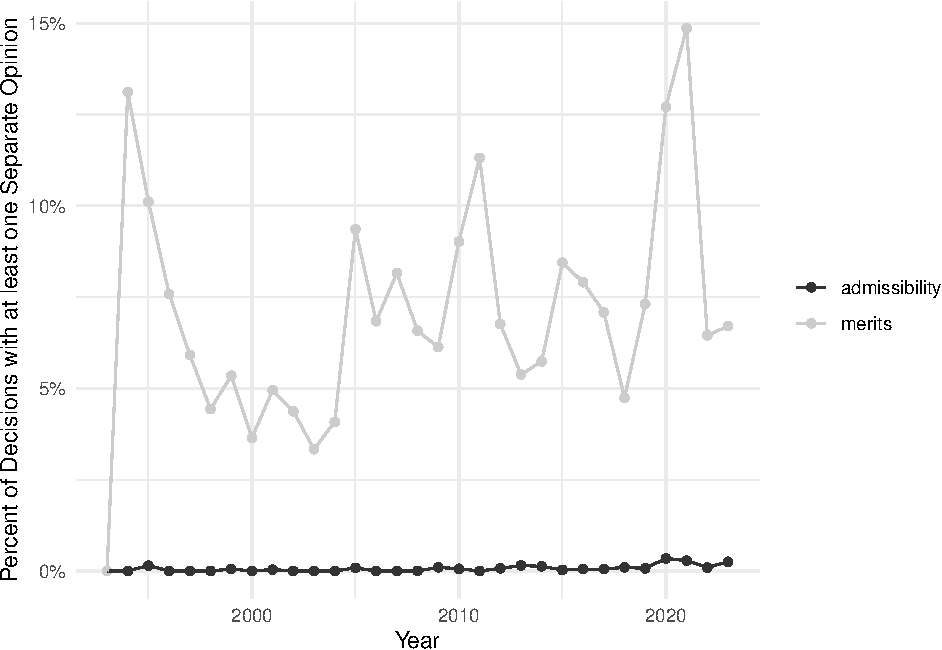
\includegraphics{separate_opinions_files/figure-latex/separate-opinion-ratio-1.pdf}
\caption{Percentage of Decisions with at least one Separate Opinion}
\end{figure}

We skip the first decade of the CCC as the data on it are rather
incomplete and inconsistent: For example, very few decisions contain the
information on the composition in the text and many do not contain the
name of the dissenting judge at all. We also limit our analysis until
the end of 2022 as the CCC entered its 4th term in 2023 and started to
undergo a complete personal change.

The final dataset for analysis contains 4621 decisions of the CCC. Table
@ref(tab:overalltable). reveals that out of them, 81.2\% are decisions
by the 3-member chambers on merits, around 9.2\% are plenum decisions on
merits and the remaining 9.6\% are plenum decisions on admissibility. At
least one separate opinion contain 4.3\% decisions out of the 3-member
decisions, 11.2\% decisions of the plenum decisionson admissibility, and
39.4\% decisions of the plenum decisions on merits.

\begin{longtable}[t]{llrll}
\caption{\label{tab:overalltable}Summary statistics for the whole dataset}\\
\toprule
\textbf{Formation} & \textbf{Grounds} & \textbf{Count} & \textbf{\%} & \textbf{\% with at least One Separate Opinion}\\
\midrule
Chamber & merits & 3862 & 81.2\% & 4.3\%\\
Plenum & admissibility & 456 & 9.6\% & 11.2\%\\
Plenum & merits & 436 & 9.2\% & 39.4\%\\
\bottomrule
\end{longtable}

\hypertarget{operationalization}{%
\subsection{Operationalization}\label{operationalization}}

We now discuss how we operationalized the variables included in our
hypotheses. We start with the dependent variables, then we move on to
the explanatory variables and finish with control variables.

\hypertarget{dependent-variable-a-separate-opinion}{%
\subsubsection{Dependent variable: a separate
opinion}\label{dependent-variable-a-separate-opinion}}

We conceptualize our dependent variable as the information whether a
justice attached a separate opinion to a decision or not.\footnote{Unlike
  Wittig we do not call our dependent variable a judge's vote, as that
  refers to a slightly different thing within the CCC context. A judge
  may vote against the majority opinion but since they are not mandated
  to write a separate opinion, these do not necessarily overlap.
  Similarly, a judge may vote for a disposition of a case and still
  attach a concurrence separate opinion.} Our dependent variable
\emph{separate opinion} is thus a dummy variable that has two
categories: either a justice did attach a separate opinion (1) or she
did not (0) in any given case .

We do not distinguish between a concurrence and a full dissent. The
reason is two-fold: practical and theoretical. Theoretically, the
difference between the two lays only in the disposition of the case. The
justices may equally disagree on the interpretation of legal rules,
thus, in the case-space model terms
(\protect\hyperlink{ref-landaDisagreementsCollegialCourts2007}{Landa and
Lax 2007--2008}; \protect\hyperlink{ref-laxNewJudicialPolitics2011}{Lax
2011}), the judge cut points in any given case differ even when a
justice attaches ``only'' concurrence. The difference is that in the
cases containing concurrence, the case facts may have completely
accidentally fallen on the same side both of the concurring judge as
well as the majority, whereas in the cases containing a dissenting
opinion, the case fell in between the cut points. We do not consider
this phenomenon as theoretically interesting. Practically, it was
impossible to distinguish between the two categories as some decisions
simply do not contain the information whether a separate opinion was a
concurring or dissenting opinion.

\hypertarget{explanatory-variables}{%
\subsubsection{Explanatory variables}\label{explanatory-variables}}

\hypertarget{disagreement-potential}{%
\paragraph*{Disagreement potential}\label{disagreement-potential}}
\addcontentsline{toc}{paragraph}{Disagreement potential}

From the theoretical perspective it may be expected that the potential
for disagreement varies across cases. In some cases, the disagreement
potential is higher and, thus, the probability of a separate opinion is
higher than in the cases with lower potential for disagreement. More
specifically, based on our theory we expect the potential for
disagreement to be captured by two characteristics of any given case:
(1) its legal complexity and (2) its controversy or in terms of Epstein
and Segal
(\protect\hyperlink{ref-epsteinMeasuringIssueSalience2000}{2000}) issue
salience.

\hypertarget{complexity}{%
\subparagraph*{Complexity}\label{complexity}}
\addcontentsline{toc}{subparagraph}{Complexity}

As Corley, Steigerwalt, and Ward
(\protect\hyperlink{ref-corleyPuzzleUnanimityConsensus2013}{2013}), p70
argue and empirically measure, complexity of a case leads to less
certainty and more ambiguity for the justices, which leads to a higher
probability of disagreement. The authors define legal complexity as the
number of legal issues a case has to address. True to the Corley,
Steigerwalt, and Ward
(\protect\hyperlink{ref-corleyPuzzleUnanimityConsensus2013}{2013})
study, our operationalization of complexity relies on the assumption
that the more legal issues there are in any given case, the higher the
number of references to other laws and caselaw in the text of the
corresponding decision. What's more, we are able to distinguish between
legal issues at the constitutional and ordinary level.

The variable \emph{concerned acts} captures the number of concerned
ordinary legal acts on the legal-act level, the variable \emph{concerned
constitutional acts} captures the number of articles of the
constitutional legal acts (mostly the Czech Constitution and the Charter
of Fundamental Rights and Freedoms) and variable \emph{caselaw} captures
the number of citations to its own caselaw. The information on the first
two variables is based on the metadata provided by the CCC, the last is
based on the regular expressions search of the text of the decisions.

\begin{longtable}[t]{llll}
\caption{\label{tab:unnamed-chunk-1}Correlations between Independent Variables of Case Complexity}\\
\toprule
\textbf{Variable} & \textbf{1} & \textbf{2} & \textbf{3}\\
\midrule
1. \# of Ordinary Acts & — & — & —\\
2. \# of Constitutional Articles & .35 & — & —\\
3. \# of CCC References & .32 & .48 & —\\
\bottomrule
\multicolumn{4}{l}{\rule{0pt}{1em}\textit{Note.} Correlation was calculated using the Spearman Correlation Coefficient.}\\
\end{longtable}

The first two variables we believe to be sufficiently different from
each other: a typical right to fair proceedings case may concern only
one constitutional article (the article 36 of the Charter) but many
legal acts, whereas a typical separation of powers case concerning the
Parliament concerns many constitutional articles but only few ordinary
laws. On the other hand, the number of (concerned) constitutional acts
and references to the CCC caselaw may be correlated. We therefore run
diagnostics, which reveal that the citations to CCC caselaw and the
number of references to constitutional acts are rather correlated.
Because we believe the number of cited constitutional articles to better
reflect the number of legal issues than the number of references to CCC
case-law, in our final model we include only that variable.

\hypertarget{controversyissue-salience}{%
\subparagraph*{Controversy/Issue
salience}\label{controversyissue-salience}}
\addcontentsline{toc}{subparagraph}{Controversy/Issue salience}

In a similar vein, certain typically value-laden issues may generate
more disagreement even if they raise only one or few legal questions.
Epstein and Segal
(\protect\hyperlink{ref-epsteinMeasuringIssueSalience2000}{2000})
distinguish between two types of issue salience. Retrospective issue
salience is how a particular issue is viewed in hindsight, regardless of
whether the actors at the time regarded it so. Contemporaneous salience
than captures the stance of the relevant actors, the CCC justices in our
cases, on the issue. While we are interested in the latter, it is not
obvious as to how exactly can such an information be captured. Epstein
and Segal
(\protect\hyperlink{ref-epsteinMeasuringIssueSalience2000}{2000}) reject
all the typically employed proxies for issue salience such as the number
of articles in law review that a case generated or the number of
citations a case generated. Instead, they propose a novel unbiased
transparent measure of issue salience: whether a SCOTUS decision made it
to the front-page of the New York Times newspaper. Unfortunately,
practically all of the measures are hard to transfer to a non-US
context. We cannot exactly pinpoint a similar newspaper as New York
Times in Czechia. Therefore, we need to rely on another measure of issue
salience/case controversy.

In her thesis, Wittig
(\protect\hyperlink{ref-wittigOccurrenceSeparateOpinions2016}{2016})
selected a number of subject matters she deemed as particularly
controversial. In the CCC context, there are a number of issue that have
been deemed as controversial by the Czech legal scholarship. Typically,
the restitution cases or cases concerning fundamental human rights have
been coined as rather controversial. The CCC dataset contains a table
\emph{subject\_matter}, which contains the subject matter of any given
case (a discrimination case, a separation of powers case and alike) and
information on the area of constitutional law that the case pertains
(the right to fair trial, the right of freedom of speech).

Following Wittig's method, we coded the topics as controversial when
they concern any of the following subject matters: discrimination,
expropriation, restitution, the property of church, sexual orientation,
the protection of consumer, fundamental human rights, social and
cultural rights, the right of property, the freedom of speech, and the
separation between the church and state. Therefore, the variable
\emph{controversial} is a dummy variable, which takes the value of 1
when the given case falls in any of the previously mentioned categories
or it takes the value 0 when it does not.

\hypertarget{norm-identification}{%
\paragraph*{Norm-identification}\label{norm-identification}}
\addcontentsline{toc}{paragraph}{Norm-identification}

Secondly, our theory generated a second expectation: a relationship
between adherence to the norm of consensus and the likelihood of a
separate opinion. The adherence to the norm of consensus depends on
self-identification and on self-perception of the judges: ``being part
of the system of the judiciary influences identification with the
organization's goals and it shapes considerably the judges' perception
of how to behave.''
(\protect\hyperlink{ref-wittigOccurrenceSeparateOpinions2016}{Wittig
2016, 100}).

Theoretically, we expect the adherence to the norm of consensus to
depend on one's career choices. The actors socialized within the
judiciary and its values are more likely to adhere to them than their
peers who entered the CCC from the legal practice, from politics, or
from anywhere outside the judicicary
(\protect\hyperlink{ref-wittigOccurrenceSeparateOpinions2016}{Wittig
2016, 84--87}.).

\begin{figure}
\centering
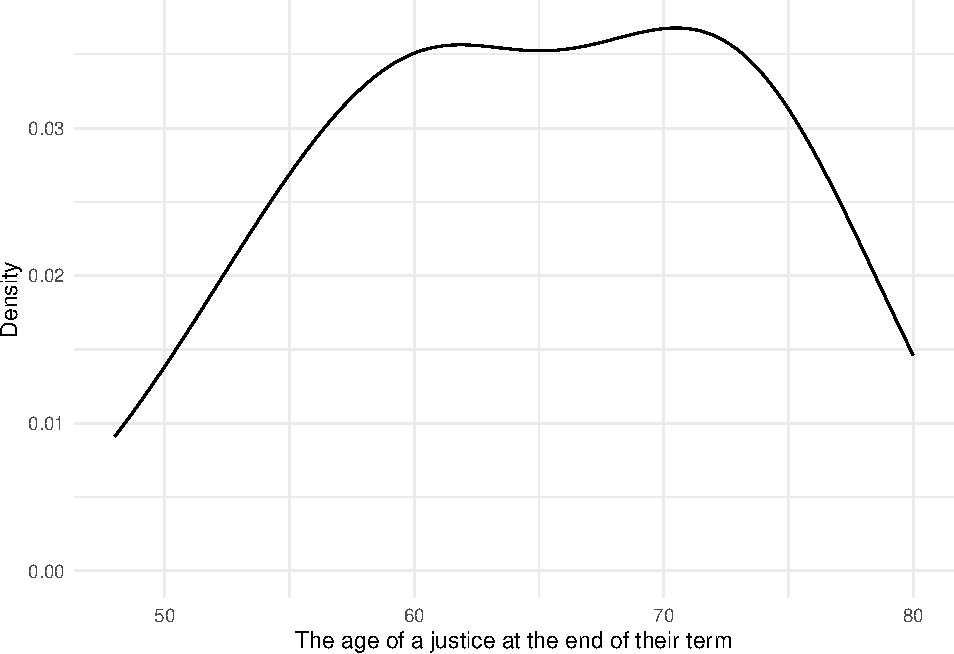
\includegraphics{separate_opinions_files/figure-latex/age-distribution-1.pdf}
\caption{Kernel density of justices' ages at the end of their terms.}
\end{figure}

Wittig confirms the theoretical intuition empirically as well but she
operationalizes the norm-identification as the justices' career choice
after their term. The justices that chose to stay within judiciary or go
back to being scholars are expected to more strongly identify with the
norm of consensus, whereas the justices' that made different career
choice are less likely to identify with the norm of consensus.
Unfortunately, such a measure does not fit the CCC context. As the table
@ref(fig:age-distribution), CCC justices start their term usually at the
end of their career and a considerable part of them ends their term in
their 70s, well past the retirement age in Czechia. Given that the
retirement age of judges 65 years of age, we expect majority of the CCC
justices to simply retire after their terms.

\begin{figure}
\centering
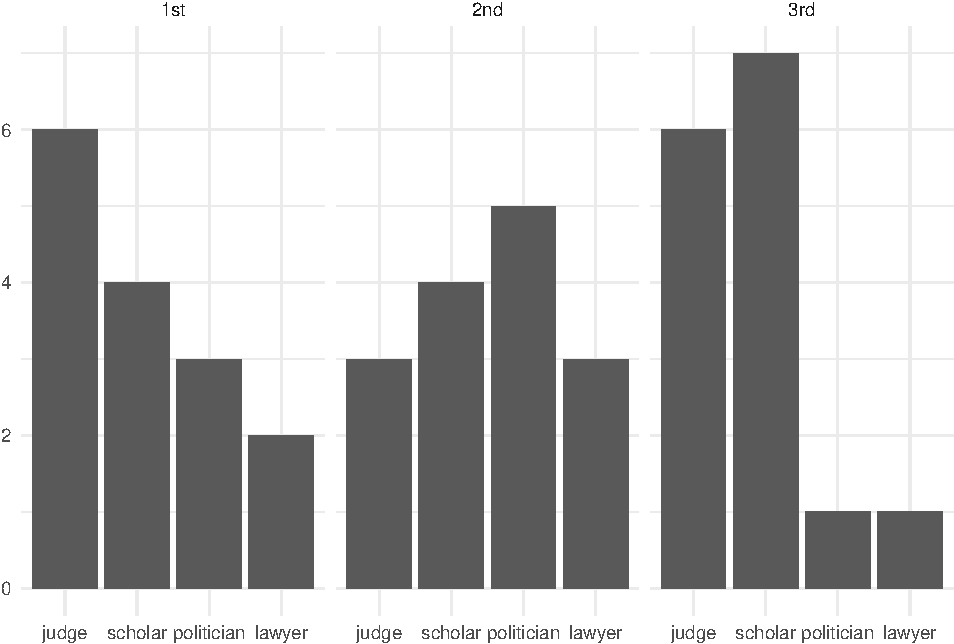
\includegraphics{separate_opinions_files/figure-latex/unnamed-chunk-2-1.pdf}
\caption{The distribution of professions of the CCC justices across its
3 terms.}
\end{figure}

Therefore, instead of operationalizing the norm-identification as the
profession after their term, we operationalize it as the last profession
before they entered the CCC. Viewed this way, Garoupa, Salamero-Teixidó,
and Segura
(\protect\hyperlink{ref-garoupaDisagreeingPrivateDissenting2022}{2022})
have found evidence that the individual decision to attach a separate
opinion of the judges on the Spanish Council of State depends on the
justice's professional background. The division does not cut across as
we would theoretically expect: only former politicians seem to be less
likely to attach a separate opinion, while former judges and lawyers
seem to be more likely to attach a separate opinion.

Quite handily, the CCC dataset contains such an information on the last
profession before the CCC justices took up their office. In the dataset,
the variable \emph{judge\_profession} contains the information on the
justices' previous career choices and can take up the values of judge,
scholar, politician, or lawyer. We can observe that the distribution of
the professions has changed across time. For our purposes, we flatten
the original variable into 2 levels. The variable \emph{profession} is
coded either as ``within'' if the justice previously served as a judge
or ``outside'' if they came from the other three professions.

\hypertarget{time-in-office}{%
\paragraph*{Time in office}\label{time-in-office}}
\addcontentsline{toc}{paragraph}{Time in office}

The effects of the CCC justices' profession should according to our
theoretical expectations vary depending on the time the judges have
spent in their office. The closer to them taking up the office, the
effects of their preceding profession should be more pronounced.
Similarly, according to the collegiality costs hypothesis, the
dissenting behavior of justices should vary across time. Namely,
justices are expected to dissent less likely at the beginning of their
terms, as the collegiality costs are higher, and to dissent more likely
at the end of their terms, as the collegiality costs of the disagreement
are lower. We capture the \emph{time in office} variables as the number
of months a justice has left until their end of mandate at the date of
the decision. That allows us to account both for the collegiality costs
hypothesis as well as the difference between professions hypothesis.

\hypertarget{workload}{%
\paragraph*{Workload}\label{workload}}
\addcontentsline{toc}{paragraph}{Workload}

Similarly to the study of Brekke, Naurin, et al.
(\protect\hyperlink{ref-brekkeThatOrderHow2023}{2023}) on workload at
the CJEU, we operationalize \emph{workload} as the number of pending
unfinished cases that any given judge has in the moment of any given
decision as a judge rapporteur. We firstly mined the compositions of
panels as well as the plenary from the text of the decision. We then
calculated the number of unfinished cases each judge had at the time of
any given decision as a judge rapporteur using the date of submission
and of decision of a case. The mean number of pending cases of any
justice as a judge rapporteur is 107.5295153, with quite a large
standard deviation of 54.3803111. The highest number of pending cases in
the dataset is 306 in the case of the justice Radovan Suchánek, whose
work ethic has already become a topic of scholarly discussion
(\protect\hyperlink{ref-chmelCoOvlivnujeUstavni2021}{Chmel 2021}).

\begin{longtable}[]{@{}lrrrrrrr@{}}
\caption{Summary statistics for the workload variable}\tabularnewline
\toprule\noalign{}
& Mean & SD & P0 & P25 & P50 & P75 & P100 \\
\midrule\noalign{}
\endfirsthead
\toprule\noalign{}
& Mean & SD & P0 & P25 & P50 & P75 & P100 \\
\midrule\noalign{}
\endhead
\bottomrule\noalign{}
\endlastfoot
workload & 108 & 54 & 0 & 63 & 103 & 145 & 306 \\
\end{longtable}

One looming issue arises that needs to be addressed and may introduce
bias. Not every unfinished pending case is the same. Different judges
may cope with the increasing workload differently. Czech scholars have
argued that deciding cases on admissibility, which are typically shorter
and require a rather concise argumentation, may be such a coping
mechanism of overburdened judges: it allows them to expedite decisions
faster and with less effort. Thus, the same number of unfinished pending
cases of a judge that chooses the strategy of offloading their workload
burden into decisions on admissibility may not carry the same workload
as with a judge that opts for decisions on merits more often. As a
solution, we multiply the workload by a ratio of unfinished cases on
merits to admissibility.

\hypertarget{identification-strategy}{%
\subsection{Identification Strategy}\label{identification-strategy}}

The hypotheses are tested by fitting a generalized linear model
estimating the probability of a judge attaching a separate opinion with
the dependent variable following a binomial distribution.

When identifying our model, we stood before a research choice that has
been addressed differently by different researchers. As other studies on
judicial decision-making relying on observational data, the data on
judicial-decision making offers multiple potential clustering variables
to include fixed effects on. In their study of effect of french language
on the performance of the judges at the CJEU, Cheruvu
(\protect\hyperlink{ref-cheruvuHowInstitutionalConstraints2019}{2019})
used fixed effects in their model the effects both on the individual
judges as well as on the panel level. The reasoning behind fixed effects
clustered on the formation were that it ``{[}s{]}cholars argue the
number of judges sitting on a chamber is a proxy for a cases' salience
as more important cases tend to be assigned to larger chambers (e.g. R.
D. Kelemen
(\protect\hyperlink{ref-kelemenPoliticalFoundationsJudicial2013}{2013});
Larsson and Naurin
(\protect\hyperlink{ref-larssonJudicialIndependencePolitical2016}{2016})).
Including chamber fixed-effects in my models addresses both
heterogeneity in the collegial decision-making process of different
chambers of judges and implicitly controls for the number of judges
hearing a case.'' Clark, Engst, and Staton
(\protect\hyperlink{ref-clarkEstimatingEffectLeisure2018}{2018}) in
their paper studied the effect of leisure on judicial
performance.\footnote{Also measured as time for a judge to decide a case
  similarly to the Cheruvu
  (\protect\hyperlink{ref-cheruvuHowInstitutionalConstraints2019}{2019})
  study.}. They included the the author fixed effects in their
model.\footnote{Which would correspond to the judge rapporteur in our
  case.} Brekke, Fjelstul, et al.
(\protect\hyperlink{ref-brekkeCJEUDatabasePlatform2023}{2023}) in a
study on the usage of orders at the CJEU built a logistic regression
model with subject matter fixed effects.

Because in our study, we are interested in the between variance of
individual judges as well as the subject matters, it does not make sense
to include fixed effects of either cluster. In contrast to that, we are
not interested in the so-called panel effects, especially the difference
between the 15-member plenum session and the 3-member panels could
produce bias. The more controversial cases or more legally complex cases
are typically assigned to the plenum and the occurrence of separate
opinions is higher in the plenary decisions. Moreover, the behavior of
the 3-member panels varies as well. It thus makes the most sense to
include panel fixed effects as that would allow us to control for a
potentially potent source of bias. In our model, the variable
\emph{formation} captures the exact composition of the 3-member panels,
whose composition is relative unstable especially after the introduction
of system of rotations of justices in 2016, and the information whether
the case was decided by the plenum, whose composition is relatively
stable within the two terms.

Moreover, our data includes two terms of the CCC. Its second decade
roughly between 2003 and 2013 and its second decade between 2014 and
2023. Rather than including year fixed effects, we opt for the term
fixed effects. If the majority of judges sitting in a panel came from
the first term, the variable \emph{term} is then coded as ``1st'', and
if the majority of justices sitting in a panel came from the second
term, the variable takes up the value ``2st''.

\hypertarget{results}{%
\subsection{Results}\label{results}}

The results reveal quite an interesting trend at the CCC. We tested the
model under more specifications. The full model presented the best fit.
However, while excluding the disagreement potential variables produced a
significant drop in AIC, excluding the norm-identification did not.
Therefore, the norm-identification variables do not seem to carry too
much explanatory power regarding the dissenting behavior of CCC
justices.

\begin{table}
\centering
\caption{\label{tab:unnamed-chunk-3}Results from the Logit Model}
\centering
\begin{tabular}[t]{lccc}
\toprule
  & Full Model & Disagreement & Norm\\
\midrule
(Intercept) & \num{-4.111}*** & \num{-4.172}*** & \num{-4.648}***\\
 & (\num{0.235}) & (\num{0.234}) & (\num{0.218})\\
n\_concerned\_acts & \num{0.086}** & \num{0.084}** & \\
 & (\num{0.026}) & (\num{0.026}) & \\
n\_concerned\_constitutional\_acts & \num{0.165}*** & \num{0.166}*** & \\
 & (\num{0.031}) & (\num{0.031}) & \\
n\_citations & \num{0.260}*** & \num{0.256}*** & \\
 & (\num{0.025}) & (\num{0.025}) & \\
groundsadmissibility & \num{-0.627}*** & \num{-0.639}*** & \num{-1.350}***\\
 & (\num{0.113}) & (\num{0.113}) & (\num{0.099})\\
judge\_professionwithin & \num{-0.117} &  & \num{-0.042}\\
 & (\num{0.077}) &  & (\num{0.075})\\
time\_in\_office & \num{0.001} &  & \num{0.129}**\\
 & (\num{0.051}) &  & (\num{0.048})\\
controversial0 & \num{-0.513}*** & \num{-0.509}*** & \\
 & (\num{0.115}) & (\num{0.115}) & \\
workload & \num{-0.117}** & \num{-0.104}** & \\
 & (\num{0.040}) & (\num{0.038}) & \\
judge\_professionwithin × time\_in\_office & \num{-0.097} &  & \num{-0.120}\\
 & (\num{0.076}) &  & (\num{0.074})\\
SD (Intercept formation) & \num{0.970} & \num{0.991} & \num{1.048}\\
\midrule
Num.Obs. & \num{21582} & \num{21582} & \num{21582}\\
R2 Marg. & \num{0.076} & \num{0.074} & \num{0.066}\\
R2 Cond. & \num{0.282} & \num{0.287} & \num{0.300}\\
AIC & \num{6329.1} & \num{6327.7} & \num{6597.9}\\
BIC & \num{6416.9} & \num{6391.5} & \num{6645.8}\\
ICC & \num{0.2} & \num{0.2} & \num{0.3}\\
RMSE & \num{0.19} & \num{0.19} & \num{0.19}\\
\bottomrule
\end{tabular}
\end{table}

Moving on to the interpretation of the results, we find a clear support
for Hypothesis X: all the disagreement potential variables are
positively and significantly correlated with the probability of a judge
attaching a separate opinion. No matter the model specification, we
always found a clear statistical, substantive and positive relationship
between the probability of a judge attaching a separate opinion and the
number of constitutional or ordinary acts concerned and the number of
CCC caselaw references. The same applies to the controversial
value-laden topics. While such a conclusion may not come as a complete
surprise, as it is perfectly aligned with theoretical expectations, we
provide a firm evidence for it.

Our results do not support the Hypothesis X. Interestingly, unlike at
the GFCC, we do not find evidence for the norm-consensus operating
according to our theoretical expectations. Firstly, adding the
interaction term between the professional background and the time in
office does not improve the model fit. It does not carry much
explanatory power as an ANOVA test fails to reject the null hypothesis
of no difference. Secondly, neither the separate variables of
norm-identification nor the interaction term are near statistical
significance. That does not however lead to us rejecting the
identification-disagreement as a theoretical model. We believe it to be
a clear theoretical model that can guide further empirical inquiries. It
may just be the case that the proxy of the justices' profession may not
be wholly accurate or that even if it was there may simply be currently
no norm of consensus operating at the CCC.

Our results also support for Hypothesis X. Higher workload of a judge
decreases their probability of attaching a separate opinion. It thus
appears that neither the claims of Epstein, Landes, and Posner
(\protect\hyperlink{ref-epsteinWhyWhenJudges2011}{2011}) are not
unwarranted and may carry over to other contexts. The results thus
reveal that judges of the CCC give way to strategical considerations
regarding their leisure. If they're overburdened with work, they reduce
the load elsewhere, namely in the additional burden of writing separate
opinions.

Lastly, we do not find evidence for the so-called freshman's effect. The
importance CCC justices attach to collegiality costs of a separate
opinion seem to remain consistent across time as the time in office of a
justice does not carry explanatory power in our model.

\hypertarget{conclusions}{%
\section{Conclusions}\label{conclusions}}

\vspace{30pt}

\hypertarget{references}{%
\section*{References}\label{references}}
\addcontentsline{toc}{section}{References}

\hypertarget{refs}{}
\begin{CSLReferences}{1}{0}
\leavevmode\vadjust pre{\hypertarget{ref-arnoldScalingCourtDecisions2023}{}}%
Arnold, Christian, Benjamin G. Engst, and Thomas Gschwend. 2023.
{``Scaling {Court Decisions} with {Citation Networks}.''} \emph{Journal
of Law and Courts} 11 (1): 25--44. \url{https://doi.org/10.1086/717420}.

\leavevmode\vadjust pre{\hypertarget{ref-berdejoElectoralCyclesUS2017}{}}%
Berdejó, Carlos, and Daniel L. Chen. 2017. {``Electoral {Cycles} Among
{US Courts} of {Appeals Judges}.''} \emph{The Journal of Law and
Economics} 60 (3): 479--96. \url{https://doi.org/10.1086/696237}.

\leavevmode\vadjust pre{\hypertarget{ref-bielenBacklogsLitigationRates2018}{}}%
Bielen, Samantha, Ludo Peeters, Wim Marneffe, and Lode Vereeck. 2018.
{``Backlogs and Litigation Rates: {Testing} Congestion Equilibrium
Across {European} Judiciaries.''} \emph{International Review of Law and
Economics} 53 (March): 9--22.
\url{https://doi.org/10.1016/j.irle.2017.09.002}.

\leavevmode\vadjust pre{\hypertarget{ref-boydUntanglingCausalEffects2010}{}}%
Boyd, Christina L., Lee Epstein, and Andrew D. Martin. 2010.
{``Untangling the {Causal Effects} of {Sex} on {Judging}.''}
\emph{American Journal of Political Science} 54 (2): 389--411.
\url{https://www.jstor.org/stable/25652213}.

\leavevmode\vadjust pre{\hypertarget{ref-brekkeCJEUDatabasePlatform2023}{}}%
Brekke, Stein Arne, Joshua C. Fjelstul, Silje Synnøve Lyder Hermansen,
and Daniel Naurin. 2023. {``The {CJEU Database Platform}: {Decisions}
and {Decision-Makers}.''} \emph{Journal of Law and Courts}, January,
1--22. \url{https://doi.org/10.1017/jlc.2022.3}.

\leavevmode\vadjust pre{\hypertarget{ref-brekkeThatOrderHow2023}{}}%
Brekke, Stein Arne, Daniel Naurin, Urška Šadl, and Lucía López-Zurita.
2023. {``That's an {Order}! {How} the {Quest} for {Efficiency Is
Transforming Judicial Cooperation} in {Europe}.''} \emph{JCMS: Journal
of Common Market Studies} 61 (1): 58--75.
\url{https://doi.org/10.1111/jcms.13346}.

\leavevmode\vadjust pre{\hypertarget{ref-calderiaTimeConsensualNorms1998}{}}%
Calderia, Gregory A., and Christopher J. W. Zorn. 1998. {``Of {Time} and
{Consensual Norms} in the {Supreme Court}.''} \emph{American Journal of
Political Science} 42 (3): 874--902.
\url{https://doi.org/10.2307/2991733}.

\leavevmode\vadjust pre{\hypertarget{ref-cameronChapterWhatJudges2017}{}}%
Cameron, Charles M., and Lewis A. Kornhauser. 2017. {``Chapter 3: {What
Do Judges Want}? {How} to {Model Judicial Preferences}.''} SSRN
Scholarly Paper. Rochester, NY. June 2, 2017.
\url{https://doi.org/10.2139/ssrn.2979419}.

\leavevmode\vadjust pre{\hypertarget{ref-carrubbaWhoControlsContent2012}{}}%
Carrubba, Cliff, Barry Friedman, Andrew D. Martin, and Georg Vanberg.
2012. {``Who {Controls} the {Content} of {Supreme Court Opinions}?''}
\emph{American Journal of Political Science} 56 (2): 400--412.
\url{https://doi.org/10.1111/j.1540-5907.2011.00557.x}.

\leavevmode\vadjust pre{\hypertarget{ref-cheruvuHowInstitutionalConstraints2019}{}}%
Cheruvu, Sivaram. 2019. {``How Do Institutional Constraints Affect
Judicial Decision-Making? {The European Court} of {Justice}'s {French}
Language Mandate.''} \emph{European Union Politics} 20 (4): 562--83.
\url{https://doi.org/10.1177/1465116519859428}.

\leavevmode\vadjust pre{\hypertarget{ref-chmelZpravodajoveSenatyVliv2017}{}}%
Chmel, Jan. 2017. {``Zpravodajové a Senáty: {Vliv} Složení Senátu Na
Rozhodování {Ústavního} Soudu {České} Republiky o Ústavních
Stížnostech.''} \emph{Časopis Pro Právní Vědu a Praxi} 25 (4): 739.
\url{https://doi.org/10.5817/CPVP2017-4-9}.

\leavevmode\vadjust pre{\hypertarget{ref-chmelCoOvlivnujeUstavni2021}{}}%
---------. 2021. \emph{Co Ovlivňuje {Ústavní} Soud a Jeho Soudce? /}.
Vydání první. Teoretik ({Leges}). Leges,.

\leavevmode\vadjust pre{\hypertarget{ref-clarkEstimatingEffectLeisure2018}{}}%
Clark, Tom S., Benjamin G. Engst, and Jeffrey K. Staton. 2018.
{``Estimating the {Effect} of {Leisure} on {Judicial Performance}.''}
\emph{The Journal of Legal Studies} 47 (2): 349--90.
\url{https://doi.org/10.1086/699150}.

\leavevmode\vadjust pre{\hypertarget{ref-clarkLocatingSupremeCourt2010}{}}%
Clark, Tom S., and Benjamin Lauderdale. 2010. {``Locating {Supreme Court
Opinions} in {Doctrine Space}.''} \emph{American Journal of Political
Science} 54 (4): 871--90.
\url{https://doi.org/10.1111/j.1540-5907.2010.00470.x}.

\leavevmode\vadjust pre{\hypertarget{ref-corleyPuzzleUnanimityConsensus2013}{}}%
Corley, Pamela C., Amy Steigerwalt, and Artemus Ward. 2013. \emph{The
{Puzzle} of {Unanimity}: {Consensus} on the {United States Supreme
Court}}. Redwood City, UNITED STATES: Stanford University Press.
\url{http://ebookcentral.proquest.com/lib/huberlin-ebooks/detail.action?docID=1180198}.

\leavevmode\vadjust pre{\hypertarget{ref-coupetteQuantitativeRechtswissenschaft2018}{}}%
Coupette, Corinna, and Andreas M. Fleckner. 2018. {``Quantitative
{Rechtswissenschaft}.''} \emph{JuristenZeitung (JZ)} 73 (8): 379--89.
\url{https://doi.org/10.1628/jz-2018-0020}.

\leavevmode\vadjust pre{\hypertarget{ref-dworkinPoliticalJudgesRule1980}{}}%
Dworkin, Ronald M. 1980. \emph{Political Judges and the Rule of Law}.
London: British Academy.

\leavevmode\vadjust pre{\hypertarget{ref-engstEinflussParteinaheAuf2017}{}}%
Engst, Benjamin G., Thomas Gschwend, Nils Schaks, Sebastian Sternberg,
and Caroline Wittig. 2017. {``Zum {Einfluss} Der {Parteinähe} Auf Das
{Abstimmungsverhalten} Der {Bundesverfassungsrichter} -- Eine
Quantitative {Untersuchung}.''} \emph{JuristenZeitung} 72 (17): 816--26.
\url{https://www.jstor.org/stable/44867374}.

\leavevmode\vadjust pre{\hypertarget{ref-epsteinChoicesJusticesMake1997}{}}%
Epstein, Lee, and Jack Knight. 1997. \emph{The {Choices Justices Make}}.
SAGE. \url{https://books.google.com?id=hSnom2h2_zUC}.

\leavevmode\vadjust pre{\hypertarget{ref-epsteinStrategicRevolutionJudicial2000}{}}%
---------. 2000. {``Toward a {Strategic Revolution} in {Judicial
Politics}: {A Look Back}, {A Look Ahead}.''} \emph{Political Research
Quarterly} 53 (3): 625--61.
\url{https://doi.org/10.1177/106591290005300309}.

\leavevmode\vadjust pre{\hypertarget{ref-epsteinWhyWhenJudges2011}{}}%
Epstein, Lee, William M. Landes, and Richard A. Posner. 2011. {``Why
({And When}) {Judges Dissent}: {A Theoretical And Empirical
Analysis}.''} \emph{Journal of Legal Analysis} 3 (1): 101--37.
\url{https://doi.org/10.1093/jla/3.1.101}.

\leavevmode\vadjust pre{\hypertarget{ref-epsteinMeasuringIssueSalience2000}{}}%
Epstein, Lee, and Jeffrey A. Segal. 2000. {``Measuring {Issue
Salience}.''} \emph{American Journal of Political Science} 44 (1):
66--83. \url{https://doi.org/10.2307/2669293}.

\leavevmode\vadjust pre{\hypertarget{ref-fjelstulEvolutionEuropeanUnion2019}{}}%
Fjelstul, Joshua C. 2019. {``The Evolution of {European Union} Law: {A}
New Data Set on the {\emph{Acquis Communautaire}}.''} \emph{European
Union Politics} 20 (4): 670--91.
\url{https://doi.org/10.1177/1465116519842947}.

\leavevmode\vadjust pre{\hypertarget{ref-fjelstulHowChamberSystem2023}{}}%
---------. 2023. {``How the {Chamber System} at the {CJEU Undermines}
the {Consistency} of the {Court}'s {Application} of {EU Law}.''}
\emph{Journal of Law and Courts}, 717422.
\url{https://doi.org/10.1086/717422}.

\leavevmode\vadjust pre{\hypertarget{ref-fjelstulTimelyAdministrationJustice2022}{}}%
Fjelstul, Joshua C., Matthew Gabel, and Clifford J. Carrubba. 2022.
{``The Timely Administration of Justice: Using Computational Simulations
to Evaluate Institutional Reforms at the {CJEU}.''} \emph{Journal of
European Public Policy}, August, 1--22.
\url{https://doi.org/10.1080/13501763.2022.2113115}.

\leavevmode\vadjust pre{\hypertarget{ref-foxallWhatJudgesMaximize2004}{}}%
Foxall, Gordon R. 2004. {``What Judges Maximize:toward an Economic
Psychology of the Judicial Utility Function.''} \emph{Liverpool Law
Review} 25 (3): 177--94.
\url{https://doi.org/10.1007/s10991-004-2877-9}.

\leavevmode\vadjust pre{\hypertarget{ref-garoupaJudicialDissentCollegial2022}{}}%
Garoupa, Nuno, and Catarina Santos Botelho. 2022. {``Judicial {Dissent}
in {Collegial Courts}: {Theory} and {Evidence}.''} In \emph{Oxford
{Research Encyclopedia} of {Politics}}.
\url{https://doi.org/10.1093/acrefore/9780190228637.013.1990}.

\leavevmode\vadjust pre{\hypertarget{ref-garoupaDisagreeingPrivateDissenting2022}{}}%
Garoupa, Nuno, Laura Salamero-Teixidó, and Adrián Segura. 2022.
{``Disagreeing in Private or Dissenting in Public: An Empirical
Exploration of Possible Motivations.''} \emph{European Journal of Law
and Economics} 53 (2): 147--73.
\url{https://doi.org/10.1007/s10657-021-09713-6}.

\leavevmode\vadjust pre{\hypertarget{ref-gschwendAreJudgesPolitical2016}{}}%
Gschwend, Thomas, Sebastian Sternberg, and Steffen Zittlau. 2016. {``Are
{Judges Political Animals} After {All}? {Quasi-Experimental Evidence}
from the {German Federal Constitutional Court}.''} SSRN Scholarly Paper.
Rochester, NY. February 26, 2016.
\url{https://doi.org/10.2139/ssrn.2738512}.

\leavevmode\vadjust pre{\hypertarget{ref-hamannGermanFederalCourts2019}{}}%
Hamann, Hanjo. 2019. {``The {German Federal Courts Dataset} 1950--2019:
{From Paper Archives} to {Linked Open Data}.''} \emph{Journal of
Empirical Legal Studies} 16 (3): 671--88.
\url{https://doi.org/10.1111/jels.12230}.

\leavevmode\vadjust pre{\hypertarget{ref-hanrettyDissentIberiaIdeal2012}{}}%
Hanretty, Chris. 2012. {``Dissent in {Iberia}: {The} Ideal Points of
Justices on the {Spanish} and {Portuguese Constitutional Tribunals}.''}
\emph{European Journal of Political Research} 51 (5): 671--92.
\url{https://doi.org/10.1111/j.1475-6765.2012.02056.x}.

\leavevmode\vadjust pre{\hypertarget{ref-hanrettyJudicialDisagreementNeed2015}{}}%
---------. 2015. {``Judicial {Disagreement} Need Not Be {Political}:
{Dissent} on the {Estonian Supreme Court}.''} \emph{Europe-Asia Studies}
67 (6): 970--88. \url{https://doi.org/10.1080/09668136.2015.1054260}.

\leavevmode\vadjust pre{\hypertarget{ref-hanrettyCourtSpecialistsJudicial2020}{}}%
---------. 2020. \emph{A {Court} of {Specialists}: {Judicial Behavior}
on the {UK Supreme Court}}. Oxford University Press.
\url{https://doi.org/10.1093/oso/9780197509234.001.0001}.

\leavevmode\vadjust pre{\hypertarget{ref-horenovskyProcessMakingConstitutional2015}{}}%
Hořeňovský, Jan, and Jan Chmel. 2015. {``The Process of making the
Constitutional Court Judgements.''} \emph{Časopis pro právní vědu a
praxi} 23 (3): 302--11.
\url{https://www.ceeol.com/search/article-detail?id=780150}.

\leavevmode\vadjust pre{\hypertarget{ref-kastellecEmpiricallyEvaluatingCountermajoritarian2016}{}}%
Kastellec, Jonathan P. 2016. {``Empirically {Evaluating} the
{Countermajoritarian Difficulty}: {Public Opinion}, {State Policy}, and
{Judicial Review} Before {\emph{Roe}}{ \emph{v.} }{\emph{Wade}}.''}
\emph{Journal of Law and Courts} 4 (1): 1--42.
\url{https://doi.org/10.1086/683466}.

\leavevmode\vadjust pre{\hypertarget{ref-kelemenJudicialDissentEuropean2017}{}}%
Kelemen, Katalin. 2017. \emph{Judicial {Dissent} in {European
Constitutional Courts}: {A Comparative} and {Legal Perspective}}.
Routledge. \url{https://books.google.com?id=kXM3DwAAQBAJ}.

\leavevmode\vadjust pre{\hypertarget{ref-kelemenPoliticalFoundationsJudicial2013}{}}%
Kelemen, R. Daniel. 2013. {``The Political Foundations of Judicial
Independence in the {European Union}.''} In \emph{The {Power} of the
{European Court} of {Justice}}. Routledge.

\leavevmode\vadjust pre{\hypertarget{ref-kornhauserModelingCollegialCourts1992a}{}}%
Kornhauser, Lewis A. 1992a. {``Modeling {Collegial Courts}. {II}. {Legal
Doctrine}.''} \emph{Journal of Law, Economics and Organization} 8: 441.
\url{https://heinonline.org/HOL/Page?handle=hein.journals/jleo8&id=449&div=&collection=}.

\leavevmode\vadjust pre{\hypertarget{ref-kornhauserModelingCollegialCourts1992}{}}%
---------. 1992b. {``Modeling Collegial Courts {I}:
{Path-dependence}.''} \emph{International Review of Law and Economics}
12 (2): 169--85. \url{https://doi.org/10.1016/0144-8188(92)90034-O}.

\leavevmode\vadjust pre{\hypertarget{ref-kosarConstitutionalCourtCzechia2020}{}}%
Kosař, David, and Ladislav Vyhnánek. 2020. {``The {Constitutional Court}
of {Czechia}.''} In \emph{The {Max Planck Handbooks} in {European Public
Law}: {Volume III}: {Constitutional Adjudication}: {Institutions}},
edited by Armin von Bogdandy, Peter Huber, and Christoph Grabenwarter,
0. Oxford University Press.
\url{https://doi.org/10.1093/oso/9780198726418.003.0004}.

\leavevmode\vadjust pre{\hypertarget{ref-landaDisagreementsCollegialCourts2007}{}}%
Landa, Dimitri, and Jeffrey R. Lax. 2007--2008. {``Disagreements on
{Collegial Courts}: {A Case-Space Approach}.''} \emph{University of
Pennsylvania Journal of Constitutional Law} 10: 305.
\url{https://heinonline.org/HOL/Page?handle=hein.journals/upjcl10&id=315&div=&collection=}.

\leavevmode\vadjust pre{\hypertarget{ref-larssonJudicialIndependencePolitical2016}{}}%
Larsson, Olof, and Daniel Naurin. 2016. {``Judicial {Independence} and
{Political Uncertainty}: {How} the {Risk} of {Override Affects} the
{Court} of {Justice} of the {EU}.''} \emph{International Organization}
70 (2, 2): 377--408. \url{https://doi.org/10.1017/S0020818316000047}.

\leavevmode\vadjust pre{\hypertarget{ref-lauderdaleScalingPoliticallyMeaningful2014}{}}%
Lauderdale, Benjamin E., and Tom S. Clark. 2014. {``Scaling {Politically
Meaningful Dimensions Using Texts} and {Votes}: {SCALING POLITICALLY
MEANINGFUL DIMENSIONS}.''} \emph{American Journal of Political Science}
58 (3): 754--71. \url{https://doi.org/10.1111/ajps.12085}.

\leavevmode\vadjust pre{\hypertarget{ref-laxNewJudicialPolitics2011}{}}%
Lax, Jeffrey R. 2011. {``The {New Judicial Politics} of {Legal
Doctrine}.''} \emph{Annual Review of Political Science} 14 (1): 131--57.
\url{https://doi.org/10.1146/annurev.polisci.042108.134842}.

\leavevmode\vadjust pre{\hypertarget{ref-moyerJudicialInnovationSexual2012}{}}%
Moyer, Laura P., and Holley Tankersley. 2012. {``Judicial {Innovation}
and {Sexual Harassment Doctrine} in the {U}.{S}. {Courts} of
{Appeals}.''} \emph{Political Research Quarterly} 65 (4): 784--98.
\url{https://doi.org/10.1177/1065912911411097}.

\leavevmode\vadjust pre{\hypertarget{ref-narayanConsensualNormHigh2005}{}}%
Narayan, Paresh Kumar, and Russell Smyth. 2005. {``The {Consensual Norm}
on the {High Court} of {Australia}: 1904-2001.''} \emph{International
Political Science Review} 26 (2): 147--68.
\url{https://doi.org/10.1177/0192512105050379}.

\leavevmode\vadjust pre{\hypertarget{ref-paulikCzechConstitutionalCourt2024}{}}%
Paulík, Štěpán. 2024. {``The {Czech Constitutional Court Dataset}.''}
\emph{Forthcoming}, 15.
\url{https://github.com/stepanpaulik/ccc_dataset/blob/main/report/ANONYMIZED_The_Czech_Constitutional_Court_Dataset.pdf}.

\leavevmode\vadjust pre{\hypertarget{ref-posnerWhatJudgesJustices1993}{}}%
Posner, Richard A. 1993. \emph{What {Do Judges} and {Justices
Maximize}?: (The {Same Thing Everyone Else Does})}. Law School,
University of Chicago. \url{https://books.google.com?id=ciFUHQAACAAJ}.

\leavevmode\vadjust pre{\hypertarget{ref-posnerHowJudgesThink2010}{}}%
---------. 2010. \emph{How {Judges Think}}. Harvard University Press.
\url{https://books.google.com?id=ZVUC8riEVPQC}.

\leavevmode\vadjust pre{\hypertarget{ref-rousseyOverburdenedJudges2018}{}}%
Roussey, Ludivine, and Raphael Soubeyran. 2018. {``Overburdened
Judges.''} \emph{International Review of Law and Economics} 55
(September): 21--32. \url{https://doi.org/10.1016/j.irle.2018.02.003}.

\leavevmode\vadjust pre{\hypertarget{ref-scaliaDissents1998}{}}%
Scalia, Antonin. 1998. {``Dissents.''} \emph{OAH Magazine of History} 13
(1): 18--23. \url{https://www.jstor.org/stable/25163249}.

\leavevmode\vadjust pre{\hypertarget{ref-songerExplainingDissentSupreme2011}{}}%
Songer, Donald R., John Szmer, and Susan W. Johnson. 2011. {``Explaining
{Dissent} on the {Supreme Court} of {Canada}.''} \emph{Canadian Journal
of Political Science/Revue Canadienne de Science Politique} 44 (2):
389--409. \url{https://doi.org/10.1017/S0008423911000151}.

\leavevmode\vadjust pre{\hypertarget{ref-sunsteinAreJudgesPolitical2006}{}}%
Sunstein, Cass R., David Schkade, Lisa M. Ellman, and Andres Sawicki.
2006. \emph{Are {Judges Political}? {An Empirical Analysis} of the
{Federal Judiciary}}. Brookings Institution Press.
\url{https://www.jstor.org/stable/10.7864/j.ctt12879t7}.

\leavevmode\vadjust pre{\hypertarget{ref-wittigOccurrenceSeparateOpinions2016}{}}%
Wittig, Caroline. 2016. \emph{The {Occurrence} of {Separate Opinions} at
the {Federal Constitutional Court}}. Logos Verlag Berlin.
\url{https://doi.org/10.30819/4411}.

\end{CSLReferences}

\end{document}
